% ===================================================================
% MORNING TALK: "GPU Hardware Characteristics"
% Intro + What is a GPU? + Hands-on #1. (Unchanged content.)
% ===================================================================
\section{Introduction}

\begin{frame}{Key Question}
    \begin{itemize}
        \item What is the difference between a CPU and a GPU?
        \item Why we can use CUDA only on NVIDIA Hardware?
        \item Should I use OpenMP, SYCL or Kokkos? 
    \end{itemize}    
\end{frame}

\begin{frame}{Roadmap for my two sessions}
\begin{enumerate}
    \item \textbf{This morning --- What is a GPU?} Hardware in a nutshell:
          parallelism, the memory wall, the roofline. 
    \item \textbf{This afternoon --- Climbing the ladder}: from the low-level model
          up to SYCL / OpenMP / Kokkos, and why they are all the same idea.

\end{enumerate}

In between, the low-level ecosystem (CUDA / HIP / OpenCL).
\end{frame}

\section{What is a GPU?}                     

\begin{frame}{At the beginning was a loom\footnote{and then the Canuts, the Luddite, Engels' pause...}}

\begin{figure}
  \centering
  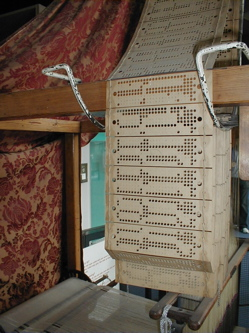
\includegraphics[width=0.27\linewidth]{Jacquard.loom.cards.jpg} 
  \caption{Late 1800s, Jacquard Machine: Threads and Warps}
\end{figure}


\end{frame}

\begin{frame}{NVIDIA in their wisdom reused some weaving terms}

\begin{figure}
    \centering
    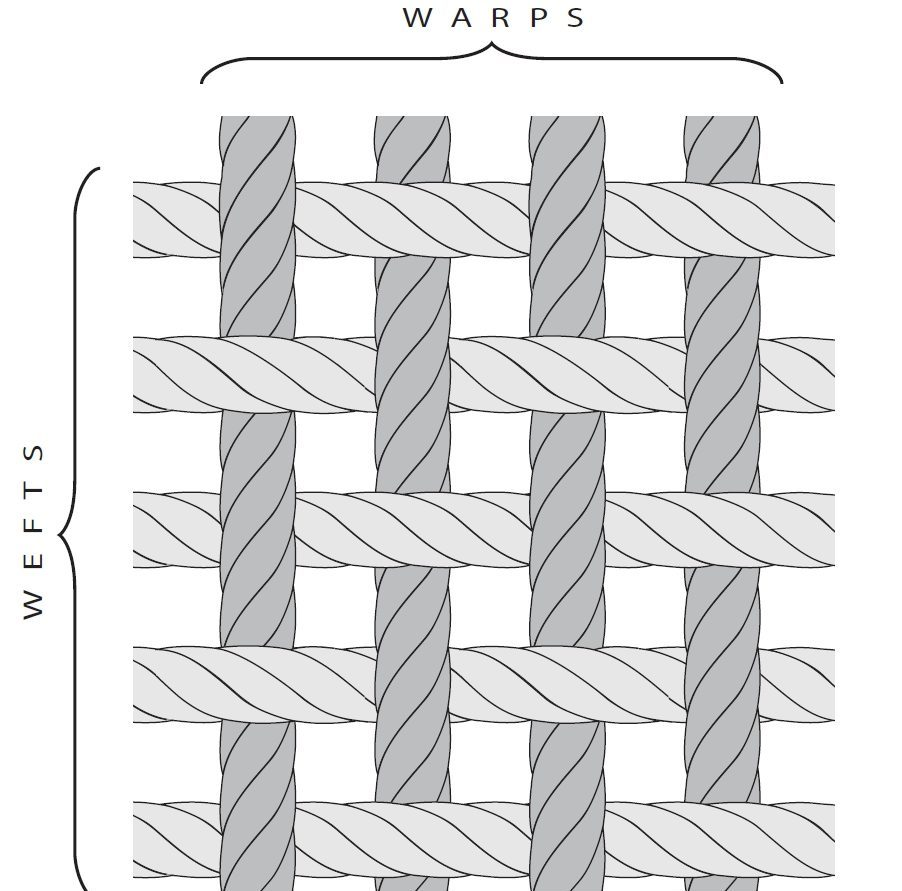
\includegraphics[width=0.30\linewidth]{wrap_thread.png}
    \caption{Warp and weft threads on a loom}
\end{figure}
Don't worry, later we will teach some less confusing terminology...
\end{frame}

\begin{frame}{And then CPU}

\begin{figure}
    \centering
    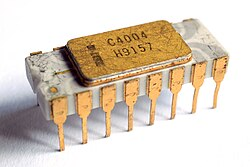
\includegraphics[width=0.5\linewidth]{image.png}
    \caption{ 1970, Intel 4004, 740 kHz, 2300 transistor}
\end{figure}

\end{frame}

\begin{frame}{How to get more performance?}
\begin{itemize}
    \item \textbf{Be Smarter} 
          \begin{itemize}
              \item Branch prediction\footnote{Speculative execution was a really good idea security wise...}, ILP (instruction level parallelism -- aka don't stall)
          \end{itemize}
    \item \textbf{Increase frequency!} Thread go faster!
          \begin{itemize}
            \item Core i9-14900K  (released in 2023) is 6 GHz
              \item One problem is power: $P \propto CV^2f$, and higher $f$ needs higher $V$ $\Rightarrow$ heat grows. 
              \item But still, still will not give you 2000x speed-up...
              
          \end{itemize}

    \item \textbf{What about doing more stuff in parallel?}
          \begin{itemize}
              \item SIMD (single instruction multiple data)
              \item More thread!
              \item This is Smart. We can always put "more" of stuff. "horizontal scaling"
          \end{itemize}
\end{itemize}

\end{frame}


\begin{frame}{Parallelism isn't new: vector computing is 50 years old}
\begin{columns}
\begin{column}{0.55\textwidth}
\begin{itemize}
    \item The \textbf{Cray-1} (1976) was a \textbf{vector} machine: one instruction
          over a whole vector of data.
    \item And then lots of CPUs work in parallel
    \item GPU is the same thing! \footnote{Kind of... with more limited synchronization}
\end{itemize}
\end{column}
\begin{column}{0.45\textwidth}
    \begin{figure}
    \centering
    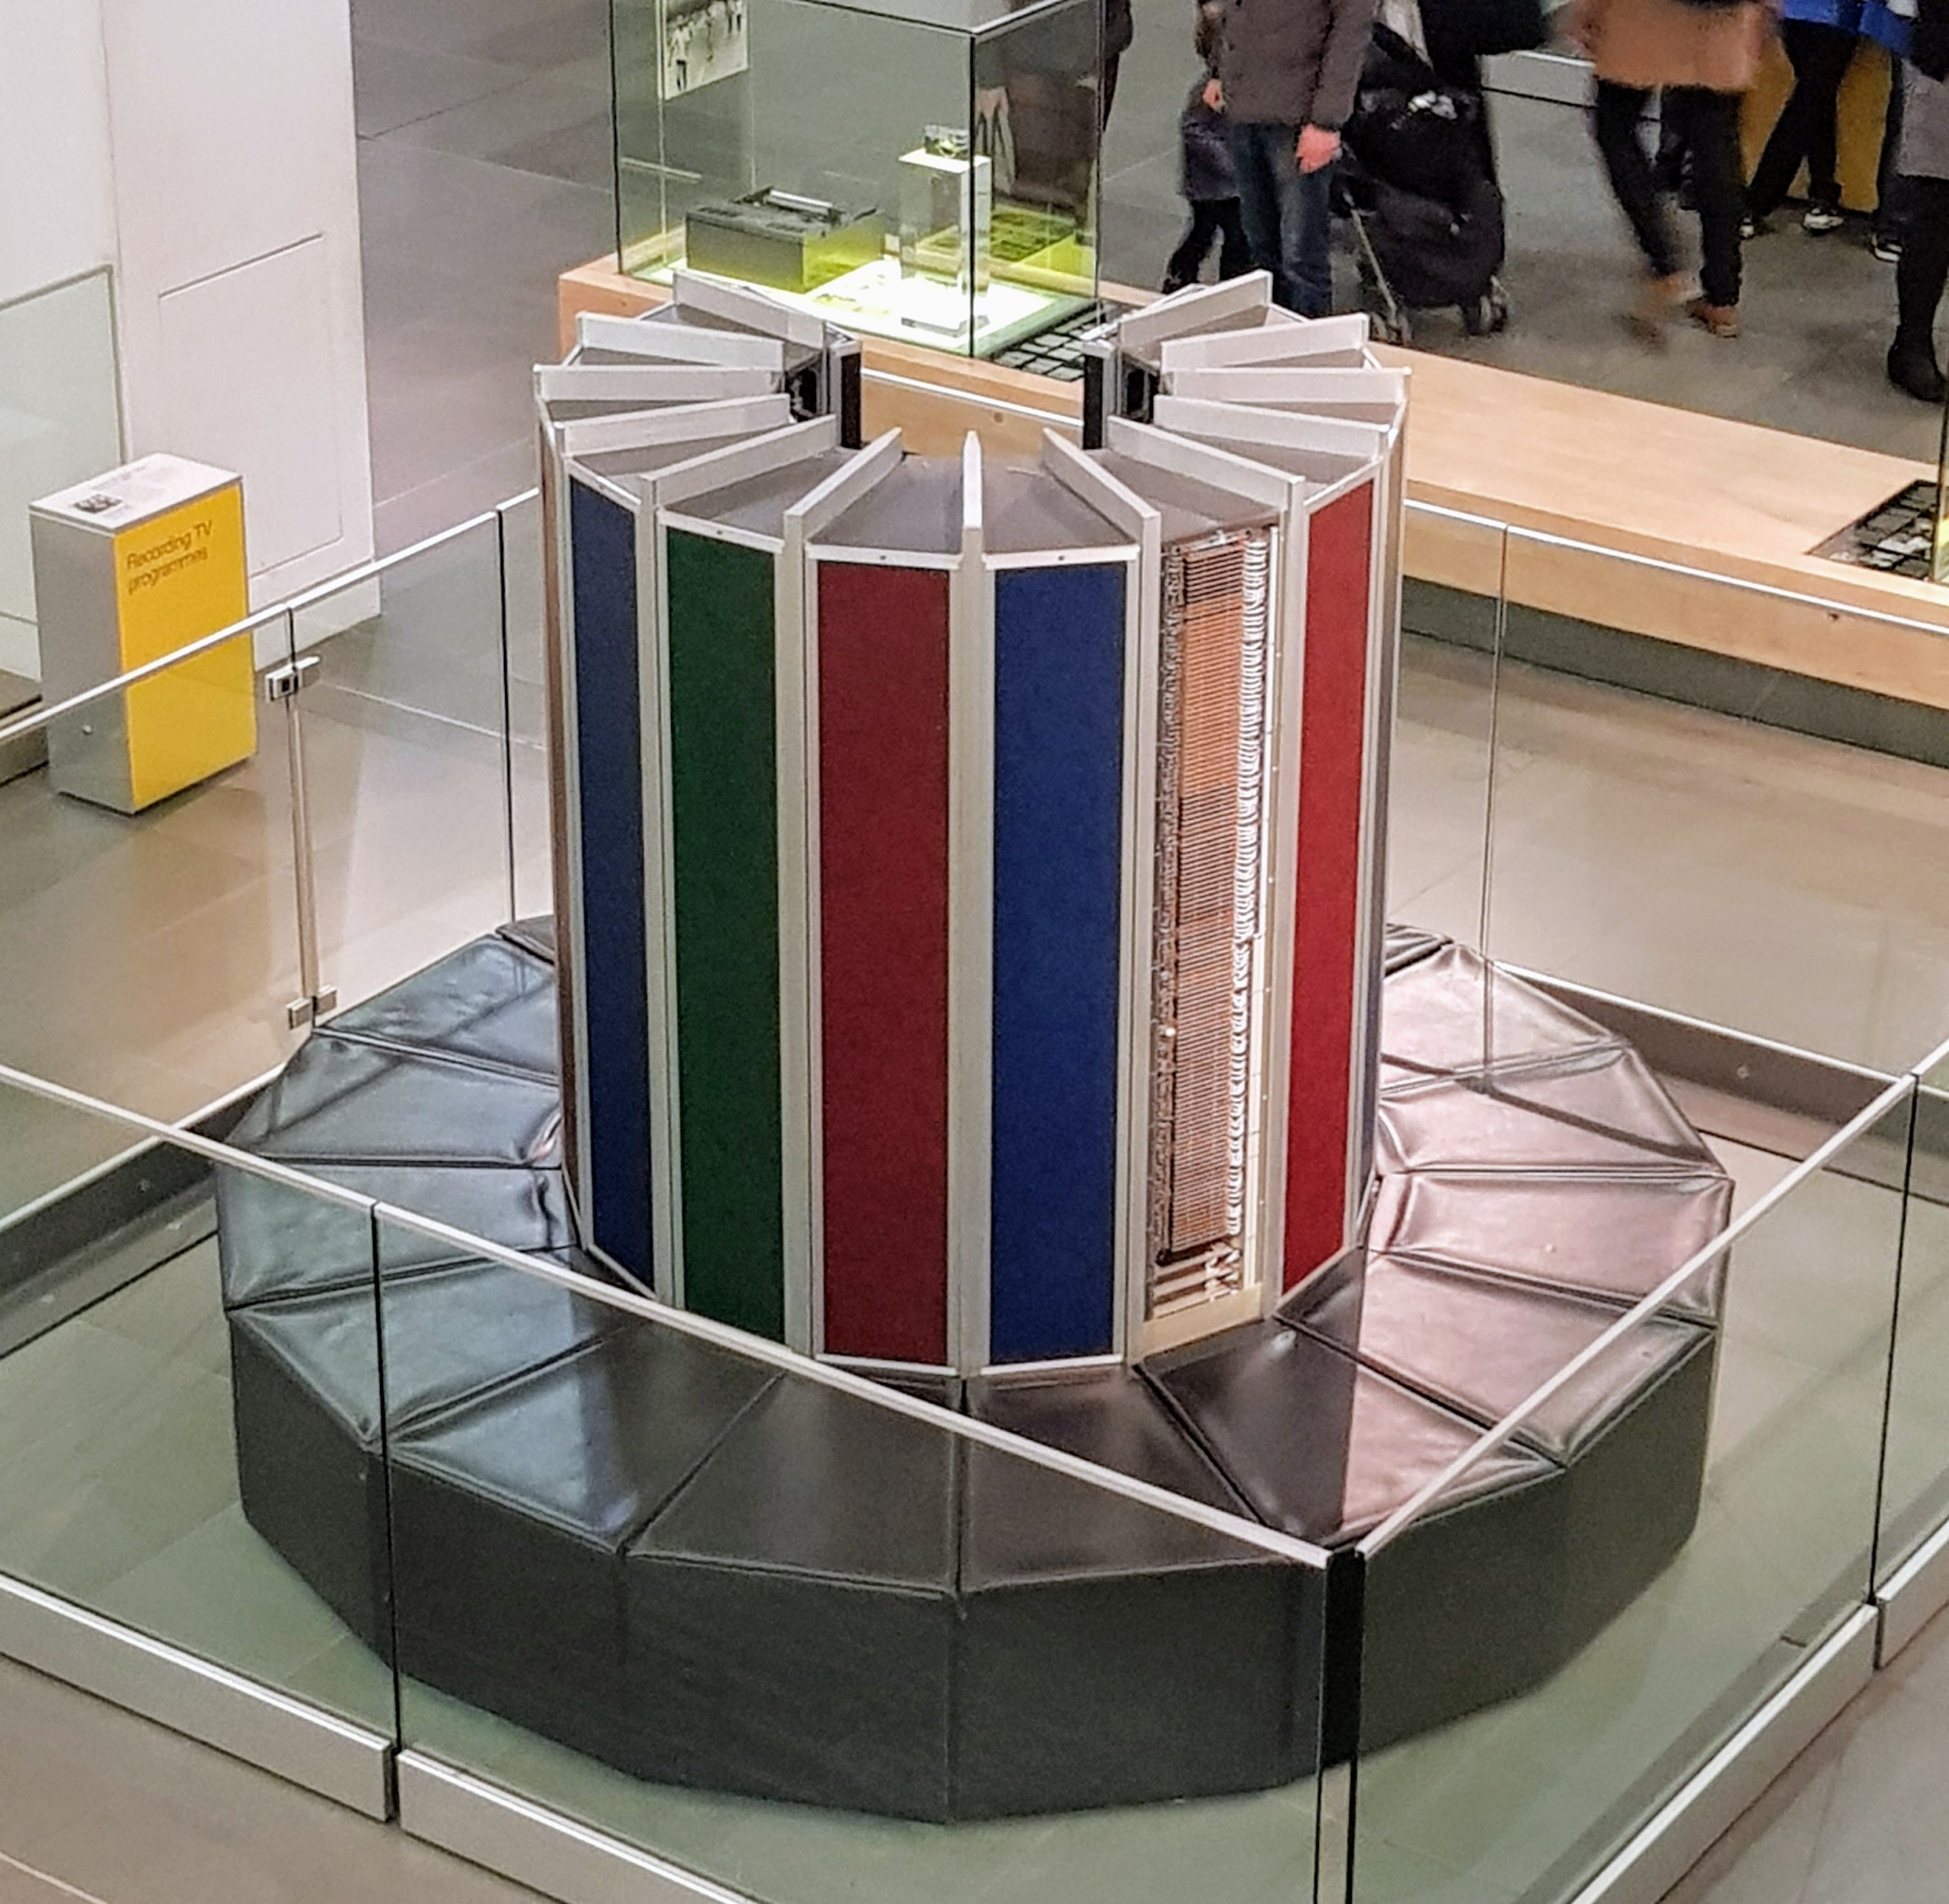
\includegraphics[height=0.7\textheight,keepaspectratio]{cray1.jpg}
    \caption{Cray-1, Science Museum London (CC BY-SA)}
    \end{figure}
\end{column}
\end{columns}

\end{frame}


\begin{frame}{And then come GPU...}

Let's just put more parallelism. No sync between them. Just for "embarrassingly-parallel" applications. Like... drawing pixels on a screen? Graphics Processing Unit
\end{frame}

\begin{frame}{It's just}


\begin{itemize}
    \item A GPU $\approx$ a very "stupid" CPU with a huge number of wide SIMD threads.
    \item And then people realised that GPU can be used to do some Linear Algebra. So why not... GP-GPU General-Purpose Graphics Processing Unit (means nothing already...)
    \item CPU followed a similar pattern, just added more threads, but smart threads. (All those ooo) and fancy synchronization (software threads can "time-slice / hyper-threading"), they can be stopped, and restarted (preemption).
\end{itemize}

And the lines are blurring: Top500 \#1 is a \textbf{pure-CPU} machine with 304
cores per socket\footnote{LineShine, Shenzhen (Top500, June 2026).}
\end{frame}




\begin{frame}{Some Terminology}

\begin{center}
\begin{tabular}{@{}ll@{}}
\toprule
\textbf{SIMD lane}        & Work on one data element \\
\textbf{SIMD instruction} & Work on multiple data at once \\
\textbf{Hardware thread}  & Execute a list of SIMD Instructions \\
\bottomrule
\end{tabular}
\end{center}

\begin{itemize}
    \item Each Hardware Thread runs some \textbf{SIMD instructions}
    \item For example Intel PVC GPU has 3{,}584 hardware threads concurrently on 512 bits wide data \footnote{Pro tips: All the HW have some register to know "where" you are running in the hardware. Not super public, but not secret either: \texttt{HW\_REG\_HW\_ID2} for AMD and \texttt{intel\_get\_slice\_id} for example}
\end{itemize}

\end{frame}

\begin{frame}{One instruction, many lanes}
\begin{center}
\begin{tikzpicture}[
    font=\scriptsize,
    lane/.style={draw, minimum width=0.75cm, minimum height=0.55cm},
    op/.style={font=\large}
]
% ---------- Scalar ----------
\node[anchor=west, font=\small] at (-1.3,2.9) {\textbf{Scalar}: 1 op $\rightarrow$ 1 result};
\node[lane, fill=ANLBlue!25]  at (0.0,2.2) {$a_0$};
\node[op] at (0.75,2.2) {$+$};
\node[lane, fill=ANLGreen!25] at (1.5,2.2) {$b_0$};
\node[op] at (2.25,2.2) {$=$};
\node[lane, fill=ANLRed!20]   at (3.0,2.2) {$c_0$};

% ---------- SIMD ----------
\node[anchor=west, font=\small] at (-1.3,1.1) {\textbf{SIMD}: 8 ops $\rightarrow$ \alert{ONE} instruction};
\foreach \i in {0,...,7} {
    \node[lane, fill=ANLBlue!25]  at (\i*0.8, 0.4) {$a_{\i}$};
    \node[lane, fill=ANLGreen!25] at (\i*0.8,-0.2) {$b_{\i}$};
    \node[lane, fill=ANLRed!20]   at (\i*0.8,-1.0) {$c_{\i}$};
}
% single-instruction annotation spanning all lanes
\draw[ANLRed, thick] (-0.45,0.7) -- (-0.45,-0.5);
\node[op, ANLRed] at (-0.75,0.1) {$+$};
\draw[-{Latex}, ANLRed, thick] (3.0,-0.5) -- (3.0,-0.7);
\node[anchor=west, ANLRed, font=\small, align=left] at (6.4,-0.1) {one instruction,\\ one cycle};
\end{tikzpicture}
\end{center}

\begin{itemize}
    \item Same opcode, same cycle --- the \textbf{lane count is the SIMD width} (here 8; PVC is 16 floats wide).
    \item A \textbf{hardware thread} just streams a list of these wide instructions.
\end{itemize}
\end{frame}

\begin{frame}{How do you get so many hardware threads? Replication (same as HPC)}

\begin{figure}
    \centering
    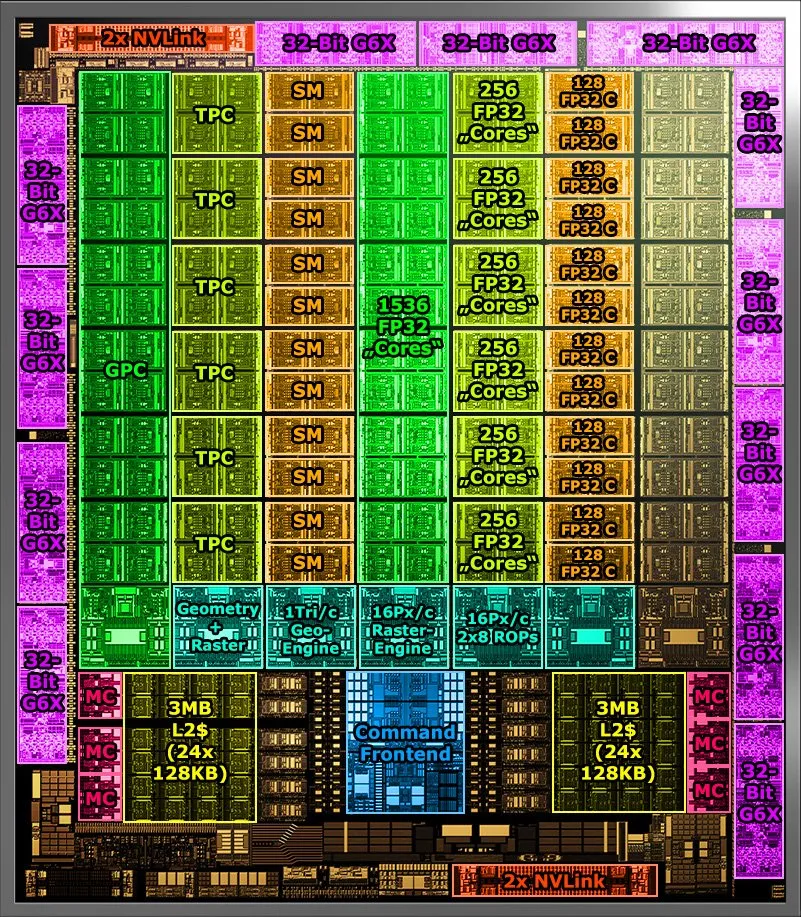
\includegraphics[width=0.40\textwidth,keepaspectratio]{locuza_ga102.png}
    \caption{Annotated NVIDIA GA102 die. Image credit: Locuza}
\end{figure}


\end{frame}

\begin{frame}{PVC Slice Example (not a real picture)}

\begin{figure}
    \centering
    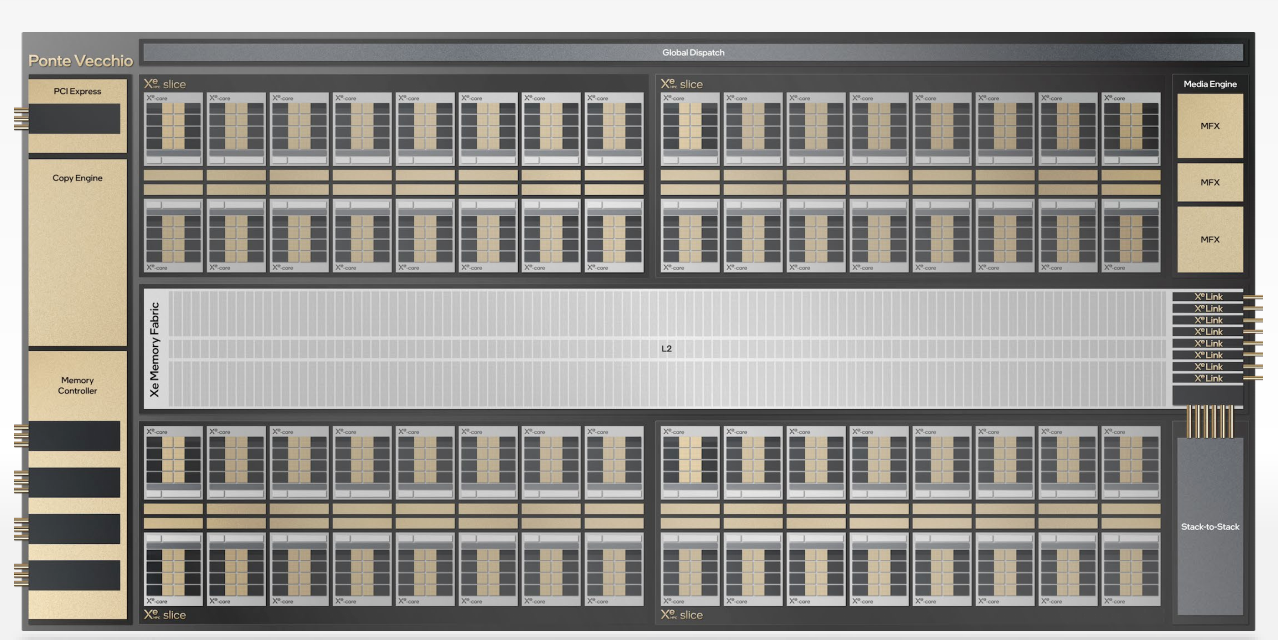
\includegraphics[width=1.0\linewidth]{pvc_slice.png}
\end{figure}
\end{frame}

\begin{frame}{Terminology}

No, I really don't want to talk about different vendors naming things differently for fun.
It's not fun.

Just some stuff share a L1, then an L2, and then nothing.  And then they are interconnected.
That's it (SM, Slice, GCD, whatever, doesn't matter. What matters is the topology)
\end{frame}

\begin{frame}{Let's still try...}

\begin{figure}
    \centering
    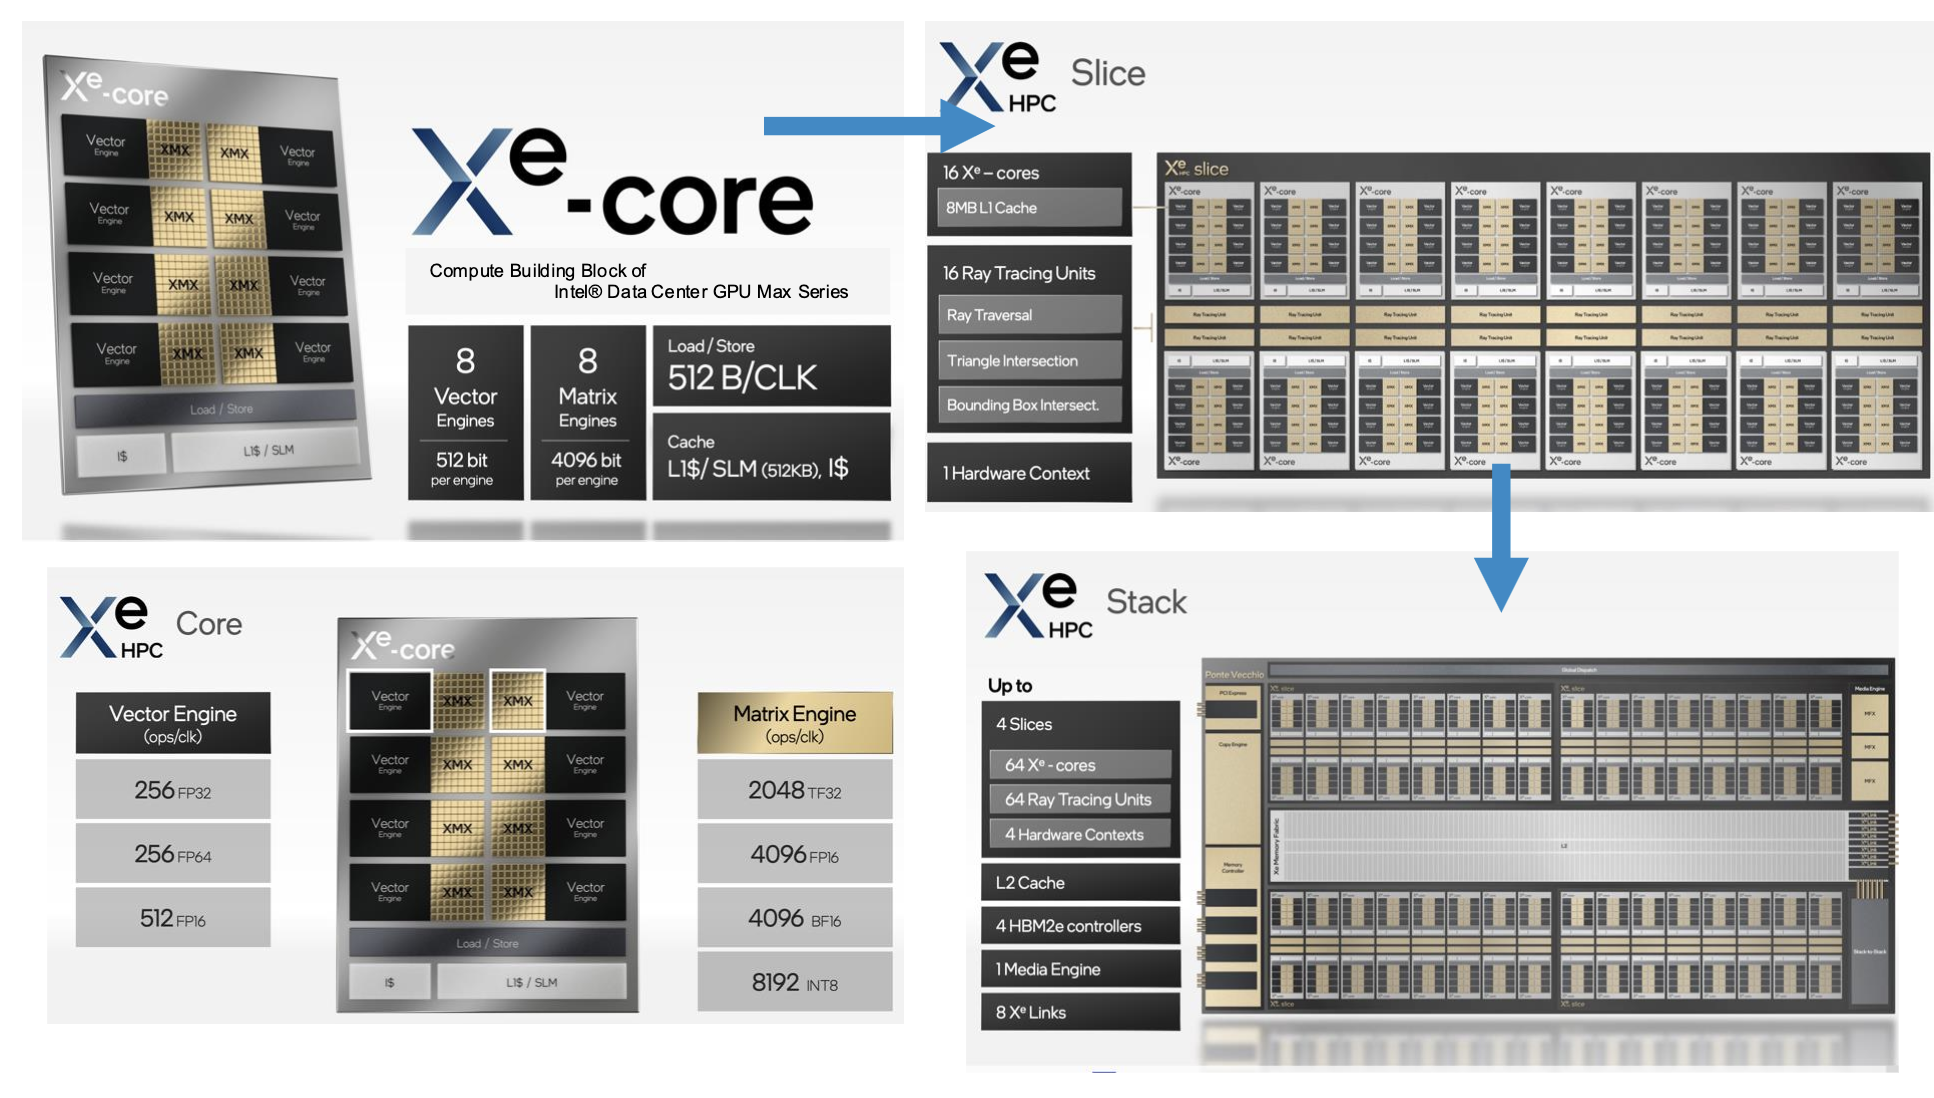
\includegraphics[width=0.8\linewidth]{intel_terminology.png}
    \caption{Intel Terminology}
\end{figure}

\end{frame}

\begin{frame}{I prefer the "logical" view}

\begin{itemize}
    \item Forget the names. What matters: \textbf{what do they share}, and
          \textbf{can they synchronize}?
    \item \textbf{Inside one Xe Core}: shared L1 / shared-local-memory, and lanes
          \alert{can sync} --- this is the compute unit (the SM / CU equivalent).
    \item \textbf{Across Xe Cores / tiles}: only an L2, then the interconnect ---
          \alert{no sync}. Same story on every vendor.
\end{itemize}

\end{frame}

\begin{frame}{Same thing, three vendors' names}

\begin{center}
\begin{tabular}{@{}llll@{}}
\toprule
\textbf{Concept} & \textbf{NVIDIA} & \textbf{AMD} & \textbf{Intel} \\
\midrule
SIMD group (lanes lock-step) & warp (32) & wavefront (64) & SIMD8/16/32 \\
\alert{Compute unit} (shares L1, \alert{can sync}) & SM & CU & Xe Core \\
Fast local memory            & shared mem & LDS & SLM \\
Whole die / tile (\alert{no sync across}) & GPU & GCD & Xe Stack \\
\bottomrule
\end{tabular}
\end{center}
\medskip
\begin{itemize}
    \item The \alert{sync boundary} is the row that matters: inside the compute
          unit you can sync + share fast memory; above it you cannot.
    \item Everything else is marketing.
\end{itemize}
\end{frame}
% === NEW  (the key restriction: no sync across hardware threads)
\begin{frame}{The one big restriction: limited synchronization}
\begin{itemize}
    \item Inside \textbf{one hardware thread}: lanes can
          sync\footnote{Obviously as most of the time they executed a lock-step}. 
    \item Across \textbf{hardware threads} running on the same core: you can sync, and have access to some fast "shared-local-memory" aka "Managed L1 cache"
    \item Between cores, it's not ok. No SYNC. There is no "global synchronization" on GPU. \footnote{I mean you can always be non-portable and do so. But threads are not "preemptable" so they cannot hit the barrier, and "make room" for other threads. They are not, because then it's not a GPU, it's a CPU. And it would be too complex / expensive, submission overhead would be huge, etc etc. Trade-off overhead}
\end{itemize}
\end{frame}

\begin{frame}{Why that restriction is a gift}
Because the hardware threads are independent, the scheduler is trivial:
\begin{itemize}
    \item If the HW has nothing to execute, just take some work.
    \item A HW thread is never \textbf{preempted} --- its registers stay live for
          its whole lifetime, so a context switch costs nothing (there is nothing
          to save/restore).
    \item So  when one HW stalls (on memory for example), another runs. That is
          how \alert{latency is hidden}, for free.
\end{itemize}
\alert{The restriction (no global sync) is exactly what buys the parallelism.}
Freedom vs.\ performance --- the GPU takes performance. Fast to schedule.
\end{frame}

\begin{frame}{Recap}
    \begin{itemize}
        \item Lots of Threads running Concurrently
        \item Not that much synchronization possible
        \item The hard thing is not really programming the GPU, it's designing an algorithm that is "embarrassingly-parallel"
        \item But at the bottom of it, this is what HPC is all about: Extracting concurrency from your algorithm/problem
    \end{itemize}
\end{frame}

% #####################################################################
\section{Performance --- Hands-on \#1}
% #####################################################################

\begin{frame}{Let's talk about performance}
Before we get started, just in case:
\begin{itemize}
    \item \textbf{FLOP} = one floating-point operation (a count). One FMA
          $a{=}b{\cdot}c{+}d$ is \textbf{2 FLOP} (but one instruction). \textbf{FLOP/S}, is FLOP per Second\footnote{and don't use FLOPS... just confusing. And I will make this mistake many times, sorry.}
\end{itemize}

We will assess the Peak FP32 of your favorite Hardware: One tile of PVC
\end{frame}

\begin{frame}{Just need to have some data}

\begin{itemize}
    \item  how many HW Threads we have,
    \item  The size of the SIMD instruction (aka how many FLOP they can do in 1 instruction)
    \item And the Frequency
    \item Then just multiply
\end{itemize}

\end{frame}

\begin{frame}[fragile]{Step 1 --- ask the hardware (\texttt{ze\_info})}
\begin{itemize}
    \item Get a node
    \item Then run \mintinline{bash}{ZE_AFFINITY_MASK=0.0 ze_info}
    \item ...
    \item  Profit (give me a number on slack). The people who have it correctly (and can explain) win a sticker!
\end{itemize}

\end{frame}
% --- Beat 1, step 1: ask the hardware
\begin{frame}[fragile]{Step 1 --- ask the hardware (\texttt{ze\_info}): Solution}
One tile (\texttt{ZE\_AFFINITY\_MASK=0.0}):
\begin{minted}{text}
Core Clock Rate             1500MHz
Physical EU SIMD Width      16      # FP32 lanes (8 for FP64)
Number EU Per SubSlice      8       # vector engines / Xe-Core
Number SubSlices Per Slice  56      # Xe-Cores per tile
Number Slices               1       # one tile
\end{minted}

Yeah, enjoy different terminology. Fun isn't it?
\end{frame}

\begin{frame}{Step 2 --- derive the theoretical peak}
Nothing magic --- just multiply the fields (FP32, one tile):
\medskip
\begin{center}
\small
$\underbrace{16}_{\substack{\text{SIMD width}\\ \text{(FP32 lanes)}}}
 \times \underbrace{8}_{\substack{\text{vector eng.}\\ \text{/ Xe-Core}}}
 \times \underbrace{56}_{\text{Xe-Cores}}
 \times \underbrace{2}_{\text{FMA}}
 \times \underbrace{1.5}_{\text{GHz}}
 \;=\; \mathbf{21{,}504}\ \text{GFLOP/s}$
\end{center}

Next question: How much of this we can reach? Any guess?
\end{frame}

\begin{frame}{Step 3 --- measure it}

\begin{itemize}
    \item I give you 3 binaries, each to measure one key characteristic.
    \item By default they use one HW thread, you can pass as argument the number you want
    \item  Enjoy compiling it. It's always one of the most fun parts...
\end{itemize}

How much? With how many HW threads used?

\medskip

Extra credit (a gift): can you write one kernel that reaches
\textbf{both} the compute and bandwidth peak at once? If somebody can do it, win a 1 dollar Cray Coin!

\end{frame}


% --- Beat 1, step 3: measure it
\begin{frame}{Step 3 --- measure all three roofs}
Run the three provided benchmarks; compare to what the hardware promised:
\begin{center}
\begin{tabular}{@{}llr@{}}
\toprule
\textbf{Benchmark} & \textbf{Roof} & \textbf{Measured} \\
\midrule
\texttt{flops} & compute (21{,}504 theo.) & \alert{21{,}427 GFLOP/s} ($\sim$99.6\%) \\
\texttt{triad} & HBM bandwidth            & \alert{$\sim$1{,}000 GB/s} \\
\texttt{pci}   & host $\leftrightarrow$ device (PCIe) & \alert{$\sim$75 GB/s} \\
\bottomrule
\end{tabular}
\end{center}
\medskip
\begin{itemize}
    \item  99\% for HBM. Easy!
    \item \textbf{Feel the gap}: HBM is $\sim$10--100$\times$ slower than compute,
          PCIe another $\sim$10--100$\times$ below HBM.
    \item  So yeah, compute fast, data-transfer slow.

\end{itemize}
\end{frame}

% === Beat 2: the FLOPs are not the bottleneck --- the memory wall
\begin{frame}{Memory wall: data movement, not FLOPs}
\begin{itemize}
    \item Compute is cheap, \textbf{data movement is expensive}: the bottleneck is
          almost always memory, not FLOPs.
    \item \textbf{Discrete GPU}: separate memory, so you must ship data over PCIe.
          Slow --- minimize transfers, keep data resident, recompute over reload.
\end{itemize}
\end{frame}

\begin{frame}{Side story: discrete accelerator $\rightarrow$ integrated}
The same cycle plays out every time, e.g.\ the floating-point unit:
\begin{itemize}
    \item \textbf{Discrete first.} The x87 math coprocessor was a separate chip
          you socketed: 8087 (with 8086/8088), 80287 (286), 80387 (386).
    \item \textbf{Then integrated.} The 486DX (1989) put the FPU on the CPU die.
          Nobody thinks of "the FPU" as a separate thing anymore.
\end{itemize}
\alert{GPUs are following the exact same path}: discrete PCIe cards today
$\rightarrow$ integrated tomorrow (APUs, MI300A, Grace-Hopper\ldots).

No silver bullet. Now we have NUMA effects. Maybe better than PCIe but not "free" either.
Locality is, always will be, key for Performance
\end{frame}


% === NEW  (arithmetic intensity: compute- vs memory-bound)
\begin{frame}{Arithmetic intensity: flop per byte}
\textbf{Arithmetic intensity} = FLOP done $/$ bytes moved. It decides whether you
are compute- or memory-bound. 

\end{frame}

% === NEW  (the money slide: the roofline, with all three roofs, measured PVC)
\begin{frame}{The roofline (one PVC tile, Single Precision)}
\begin{center}
\begin{tikzpicture}
\begin{loglogaxis}[
    width=0.82\textwidth, height=0.66\textheight,
    xlabel={arithmetic intensity (flop/byte)},
    ylabel={GFLOP/s},
    xmin=0.1, xmax=10000, ymin=10, ymax=100000,
    xtick={0.1,1,10,100,1000,10000},
    ytick={10,100,1000,10000,100000},
    tick label style={font=\scriptsize}, label style={font=\scriptsize},
    legend style={font=\scriptsize, at={(0.02,0.98)}, anchor=north west,
                  draw=none, fill=white, fill opacity=0.7, text opacity=1},
    grid=both, major grid style={black!12},
]
% Compute roof: 21427 GFLOP/s (flat)
\addplot[very thick, mDarkTeal, domain=0.1:10000, samples=2] {21427};
\addlegendentry{compute roof (21{,}427)}
% HBM roof: y = 1000 * AI, capped at compute roof (ridge at AI=21.4)
\addplot[very thick, ANLBlue] coordinates {(0.1,100) (21.4,21427) (10000,21427)};
\addlegendentry{HBM roof (1{,}000 GB/s)}
% PCIe roof: y = 75 * AI (ridge at AI=286)
\addplot[very thick, mLightBrown] coordinates {(0.133,10) (286,21427) (10000,21427)};
\addlegendentry{PCIe roof (75 GB/s)}
% Workload dots
\addplot[only marks, mark=*, mark size=2.5pt, black] coordinates {(0.17,167)};
\node[font=\scriptsize, anchor=west] at (axis cs:0.21,167) {triad (BW-bound)};
\addplot[only marks, mark=*, mark size=2.5pt, black] coordinates {(8000,21427)};
\node[font=\scriptsize, anchor=south east] at (axis cs:7000,21427) {FMA chain (compute-bound)};
% The ridge: the ONE point touching both roofs -- the extra-credit target
\addplot[only marks, mark=star, mark size=4pt, ANLGreen, very thick] coordinates {(21.4,21427)};
\node[font=\scriptsize\bfseries, ANLGreen, anchor=north west] at (axis cs:25,19000) {can you reach this?};
\end{loglogaxis}
\end{tikzpicture}
\end{center}
\vspace{-0.5em}
Below AI $\approx$20 you are HBM memory-bound; below $\sim$286 you are PCIe-bound.

\end{frame}

\begin{frame}{Just to be super clear}

AI is per byte. So for each byte you read from main memory you need to do at least 20 FLOP:
\begin{itemize}
    \item so you need at least 80 FLOP per float!  Enjoy being compute bound guys.
    \item And you have at least 7168 simd-lanes to use. If you use less, you are not fully utilizing the full compute capability of one Tile.
    \item Oh, and we have 63744 GPUs on Aurora, so you just need to use 913\_833\_984 vector lines every cycle \footnote{So if your "problem space" is lower than that, it's mathematically impossible to use Aurora at max capacity}
\end{itemize}


\end{frame}

\begin{frame}{Conclusion: GPU in a nutshell}
\begin{itemize}
    \item A wide-SIMD, latency-hiding throughput machine.
    \item The naming does matter, it's just hierarchical. You have some levels where sync is free, some where it's expensive, some where it's impossible.
    \item Fast because it is simple: no big caches, no branch prediction,
          no fancy per-lane cleverness.
    \item Gap between Memory and Flops is huge. You need to compute, compute, compute
    \item GPUs are big. And we have many of them. So please extract the maximum concurrency of your simulation. And avoid reading from main memory\footnote{cache -> data locality, re-computing}
\end{itemize}

\end{frame}

\begin{frame}{Thanks!}

I think we have a Q\&A now. 
\end{frame}

